% PREAMBLE: -
\documentclass[12pt]{article}

\usepackage{amsmath,amsfonts,mathtools,hyperref,graphicx}
\hypersetup{colorlinks=true}
\usepackage[margin=0.21in]{geometry}
\usepackage[]{microtype}
\graphicspath{{./3-img/}}

% padded box (answers)
\newcommand{\padBox}[1]{{\setlength\fboxsep{5pt}\boxed{#1}}}
% binomial exponent
\newcommand{\negBi}[3][2]{(#2- #3)^{#1}}
% large math
\newcommand*{\mL}[1]{\mbox{\Large$#1$}}
% huge math
\newcommand*{\mH}[1]{\mbox{\huge$#1$}}

\begin{document}

% SECTION: Correlation Coefficient: -

\section*{Correlation Coefficient}

\subsection*{Definition}
\paragraph{}%
A correlation coefficient is a numerical measure of some type of correlation, meaning a statistical relationship between two variables. The variables may be two columns of a given data set of observations, often called a sample, or two components of a multivariate random variable with a known distribution.

Several types of correlation coefficient exist, each with their own definition and own range of usability and characteristics. They all assume values in the range from −1 to +1, where ±1 indicates the strongest possible agreement and 0 the strongest possible disagreement. As tools of analysis, correlation coefficients present certain problems, including the propensity of some types to be distorted by outliers and the possibility of incorrectly being used to infer a causal relationship between the variables.

\subsection*{Formula}
\paragraph{For each corresponding $x$ and $y$ find the z-score for $x$:}
\begin{equation}
	\mH{%
		r = \frac{1}{n - 1}\sum
		\left(\frac{x_{i} - \bar{x}}{s_{x}}\right)
		\left(\frac{y_{i} - \bar{y}}{s_{y}}\right)
	}
\end{equation}%

\subsection*{Example}
\paragraph{Sample Data}
$x_{i}, y_{i} = (1, 1), (2, 2), (2, 3), (3, 6)$, so $\bar{x} = 2$, and $s_{x} = 0.816$, $\bar{y} = 3$, $s_{y} = 2.160$

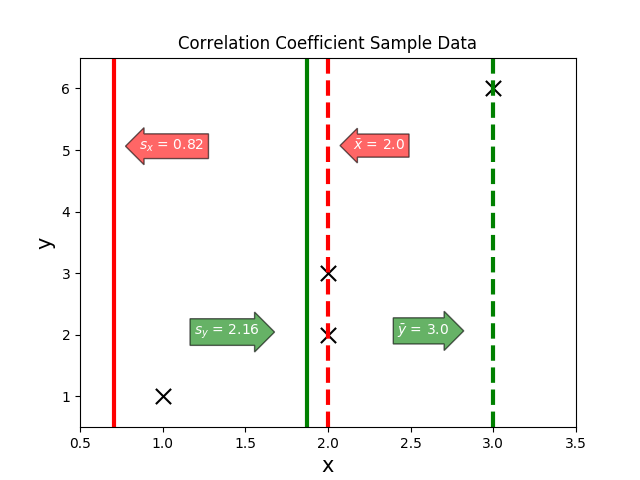
\includegraphics[scale=0.99]{correlation-coefficient-sample}
\paragraph{Calculate the sum of the product of the z-scores:}

\begin{equation}
\begin{gathered}
		r = \frac{1}{3}\sum \;\;\;%
		\left(\frac{1 - 2}{0.816}\right)\left(\frac{1 - 3}{2.16}\right) \;\;\;%
		+ \;\;\;%
		\left(\frac{2 - 2}{0.816}\right)\left(\frac{2 - 3}{2.16}\right) \;\;\;%
		+ \;\;\;%
		\left(\frac{2 - 2}{0.816}\right)\left(\frac{3 - 3}{2.16}\right) \;\;\;%
		+ \;\;\;%
		\left(\frac{3 - 2}{0.816}\right)\left(\frac{6 - 3}{2.16}\right) \;\;\;%
\end{gathered}%
\end{equation}%

\subsection*{Result}
\[\mH{r \approx 0.946}\]

\paragraph{Summary}
The closer the result is to positive one, the stronger positive correlation. The closer the result is to negative one, the stronger the negative correlation. The closer the result is to zero the weaker correlation. This result has a strong positive correlation. This can be visualized by drawing a line.

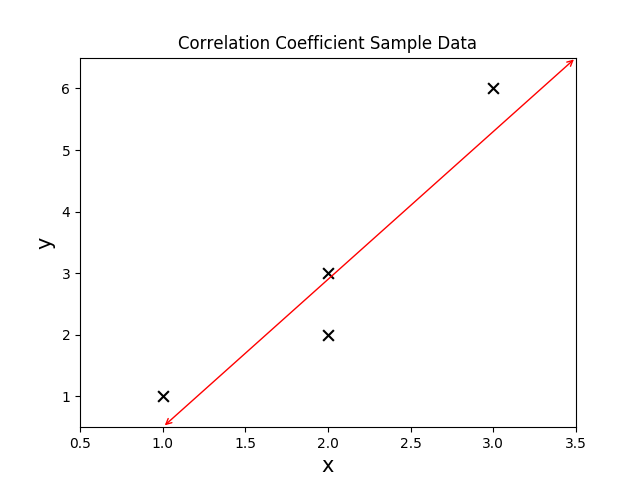
\includegraphics[scale=0.99]{correlation-coefficient-result}
\end{document}
